\chapter{Sada ukázkových testů a~jejich scénářů}
Existuje webová aplikace \emph{Převodník} dostupná z~url \url{http://oks.kiv.zcu.cz/Prevodnik/Prevodnik} se záměrnými chybami. Pro potřeby práce a~pro názornou ukázku odlišnosti přístupu k~testování webové a~desktopové aplikace byla vytvořena téměř identická aplikace Převodník pomocí technologie JavaFX, jejíž kód se nachází na přiloženém CD. Následující sada testů a~jejich scénářů se vztahuje k~těmto aplikacím, jejichž vzhled je ukázán na obrázcích \ref{PrevodnikWeb} a~\ref{PrevodnikJavaFX}.

	\begin{figure}[ht!]
		\centering
		\caption{Webová aplikace Převodník}
		\label{PrevodnikWeb}
		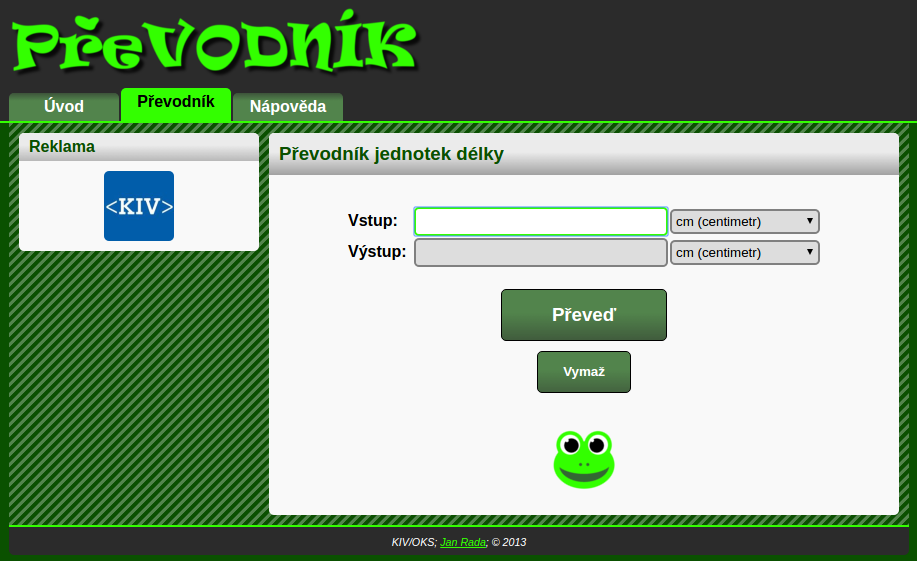
\includegraphics[width=13.5cm]{img/PrevodnikWeb.png}
	\end{figure}
	\begin{figure}[ht!]
		\centering
		\caption{Aplikace Převodník vytvořená pomocí JavaFX}
		\label{PrevodnikJavaFX}
		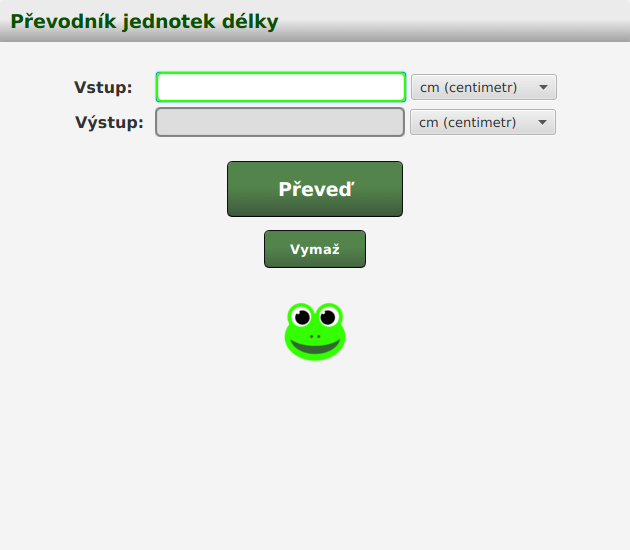
\includegraphics[width=13.5cm]{img/PrevodnikJavaFX.png}
	\end{figure}

Ze scénářů i~z~přiloženého zdrojového kódu je patrné, že přístup k~testování obou aplikací je totožný. Testy vypadají stejně jak pro desktopovou aplikaci, tak pro webovou. Jediné rozdíly nastávají ve způsobu spouštění aplikací, zacházení s~nimi a~v~cestě k~použitým řídícím screenshotům. Příčinou je to, že se jedná o~téměř identicky vypadající a~chovající se aplikace. Dále budou uvedeny vždy jen stručné ukázky testů s~vyznačenými případnými odlišnostmi.

	\section{Rozdělení testů}
	Scénáře byly rozděleny do tří částí a~každá část poté může obsahovat další skupiny, které sjednocují tematicky si blízké testy. Struktura scénářů tedy vypadá přibližně takto:
		{\renewcommand{\labelenumii}{\theenumii}
		\renewcommand{\theenumii}{\theenumi.\arabic{enumii}.}
		\begin{enumerate}
		\item Statické prvky
			\begin{enumerate}
			\item Přítomnost prvků
			\item Editovatelnost polí
			\item Úplnost výběrových seznamů
			\end{enumerate}
		\item Převody
			\begin{enumerate}
			\item Happy Day Scenario
			\item Stejné jednotky
			\item Varianty Vstup OK
			\item Vše na metr
			\item Vše z~metru
			\item Varianty Vstup CHYBA
			\item Všechny vstupy na všechny výstupy
			\item Hraniční hodnoty
			\end{enumerate}
		\item Vymazání
		\end{enumerate}}
		
	Testovací případy mají předponu \emph{TC} za níž nasleduje číslo testovacího případu a~jeho název. Pokud tedy např. testujeme úplnost výstupního výběrového seznamu, název bude \emph{TC01\_03\_02VystupniVyberovySeznam}. Číslo testovacího případu se tvoří dle jeho příslušnosti do části (TestSuite) ve výčtu výše. Patří do \emph{Úplnost výběrových seznamů} a tomu odpovídá první část čísla, \emph{01\_03}. Označení \emph{02} je pořadové číslo testu v~rámci dané kategorie.
		
	\section{Statické prvky}
	Scénáře v~této části pouze zkontrolují, zda testovaná aplikace obsahuje všechny prvky, jako např. tlačítka či vstupní pole. Dále se zkoumá, zda je vstupní pole editovatelné a~výstupní pole nikoli. Poté se zjistí, zda jsou ve výběrových seznamech obsaženy všechny položky.
	
	Následující úsek kódu \ref{statickePrvky} demonstruje, v~jakém duchu se testují statické prvky aplikace.
	\begin{lstjava}{caption={Test přítomnosti statického prvku}, label={statickePrvky}}
@Test
public void TC01_01_02VstupniTextovePole() {
  if (run) {
    try {
      assertTrue("Vstupni textove pole neexistuje",
        s.find(pngs + "labely/vstupLabel.png").
        right().grow(0, 20).exists(pngs +
        "textovaPole/vstupniTextovePole.png") !=
        null);
    } catch (FindFailed | AssertionError e) {
      s.capture().save("errors", screenshotName());
      logger.error(e.getMessage());
      fail(e.getMessage());
    }
  } else {
    logger.error("Setup failed");
    fail("Setup failed");
  }
}
\end{lstjava}
	
	\section{Převody}
	V~této části jsou zpracované funkční testy konkrétních převodů. Nejprve se provedou testy Happy Day Scenario -- scénář, kdy vše dopadne podle očekávání. Poté se zkontrolují převody mezi stejnými jednotkami, převody s~možnými korektními i~nekorektními vstupy, převody mezi všemi jednotkami a~nakonec převody s~hraničními hodnotami.
	
	Část kódu v~\ref{prevody} ukazuje, jak se mohou tvořit testy převodů.
	\begin{lstjava}{caption={Test převodu}, label={prevody}}
@Test
public void TC02_04_01PrevodCmNaM() {
  if (run) {
    try {
      s.find(pngs + "labely/vstupLabel.png").right().
        grow(0, 20).click(pngs + "textovaPole/" +
        "vstupniTextovePole.png");
      s.paste("1");
      Match hledani = s.find(pngs + "labely/" +
        "vstupLabel.png").right().grow(0, 20).find(
        pngs + "vyberoveSeznamy/vstupniVyberovy" +
        "Seznam.png");
      hledani.click();
      hledani.below().click(pngs + "vyberove" +
        "Seznamy/vstupModryCm.png");
      hledani = s.find(pngs + "labely/vystupLabel" +
        ".png").right().grow(0, 20).find(pngs +
        "vyberoveSeznamy/vystupniVyberovySeznam" +
        ".png");
      hledani.click();
      hledani.below().click(pngs + "vyberove" +
        "Seznamy/vystupM.png");
      s.click(pngs + "tlacitka/tlacitkoPreved.png");
      s.wait(pngs + "tlacitka/tlacitkoPreved.png",
        5);
      assertTrue("Ocekavano: 0.01, zjisteno neco " +
        "jineho", s.find(pngs + "labely/vystup" +
        "Label.png").right(200).grow(0, 10).exists(
        pngs + "vystupy/vystup0_01.png") != null);
    } catch (FindFailed | AssertionError e) {
      s.capture().save("errors", screenshotName());
      logger.error(e.getMessage());
      fail(e.getMessage());
    }
  } else {
    logger.error("Setup failed");
    fail("Setup failed");
  }
}
\end{lstjava}
	
	\section{Vymazání}
	V~této části se testuje funkčnosti tlačítka Vymazat. Otestuje se případ, kdy se nevyskytla chybová hláška, i~ten, kdy se vyskytla.
	
	Kód \ref{vymazani} je jednou z~možností, jak testovat správnou funkčnost tlačítka \emph{Vymazat}.
	\begin{lstjava}{caption={Test funkčnosti tlačítka \emph{Vymazat}}, label={vymazani}}
@Test
public void TC03_01_02PrevodChyba() {
  if (run) {
    try {
      s.find(pngs + "labely/vstupLabel.png").right().
        grow(0, 20).click(pngs + "textovaPole/" +
        "vstupniTextovePole.png");
      s.paste("abc");
      Match hledani = s.find(pngs + "labely/" +
        "vstupLabel.png").right().grow(0, 20).
        find(pngs + "vyberoveSeznamy/vstupni" +
        "VyberovySeznam.png");
      hledani.click();
      hledani.below().click(pngs + "vyberove" +
        "Seznamy/vstupM.png");
      hledani = s.find(pngs + "labely/vystupLabel" +
        ".png").right().grow(0, 20).find(pngs +
        "vyberoveSeznamy/vystupniVyberovySeznam" +
        ".png");
      hledani.click();
      hledani.below().click(pngs + "vyberove" +
        "Seznamy/vystupM.png");
      s.click(pngs + "tlacitka/tlacitkoPreved.png");
      s.wait(pngs + "tlacitka/tlacitkoPreved.png",
        5);
      assertTrue("Nenalezeno upozorneni o chybe", s.
        exists(pngs + "chyby/chybaNeplatneCislo") !=
        null);
      s.click(pngs + "tlacitka/tlacitkoVymaz.png");
      s.wait(pngs + "tlacitka/tlacitkoPreved.png",
        5);
      assertTrue("Vstupni pole neni prazdne", s.
        find(pngs + "labely/vstupLabel.png").right().
        grow(0, 20).exists(pngs + "textovaPole" +
        "/vstupniTextovePole.png") != null);
      assertTrue("Vystupni pole neni prazdne", s.
        find(pngs + "labely/vystupLabel.png").
        right().grow(0, 20).exists(pngs +
        "textovaPole/vystupniTextovePole.png") !=
        null);
      assertTrue("Vstupni vyberovy seznam nema" +
        "defaultni hodnotu", s.find(pngs +
        "labely/vstupLabel.png").right().grow(0, 20).
        exists(pngs + "vyberoveSeznamy/vstupni" +
        "VyberovySeznam.png") != null);
      assertTrue("Vystupni vyberovy seznam nema" +
        "defaultni hodnotu", s.find(pngs +
        "labely/vystupLabel.png").right().grow(0,
        20).exists(pngs + "vyberoveSeznamy/" +
        "vystupniVyberovySeznam.png") != null);
      assertTrue("Nalezeno upozorneni o chybe", s.
        exists(pngs + "chyby/chybaNeplatneCislo") ==
        null);
    } catch (FindFailed | AssertionError e) {
      s.capture().save("errors", screenshotName());
      logger.error(e.getMessage());
      fail(e.getMessage());
    }
  } else {
    logger.error("Setup failed");
    fail("Setup failed");
  }
}
\end{lstjava}
	
	\section{Zjištěné chyby}
	Během testování aplikace bylo zjištěno několik chyb. Jak již bylo řečeno dříve, tyto chyby jsou v~aplikaci zaneseny záměrně.
	
		\subsection{Chybné převody z~(na) decimetry}
		Pokud provádíme převod z~(případně na) decimetry, dostaneme nesprávný výsledek, viz \ref{ChybaDm}. Chování odpovídá převodu z~(na) palce.
			\begin{figure}[ht!]
				\centering
				\caption{Chybný převod z decimetru na centimetr}
				\label{ChybaDm}
				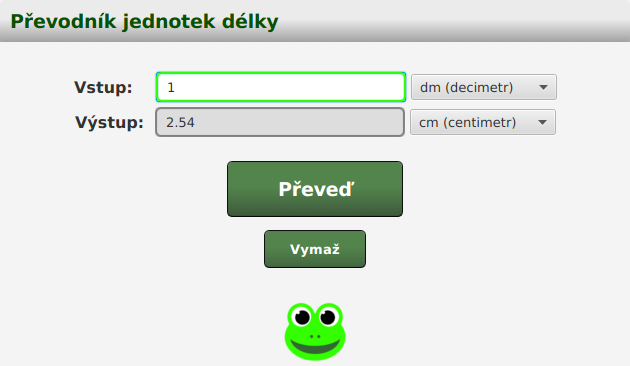
\includegraphics[width=13.5cm]{img/Chyby/Dm.png}
			\end{figure}
			\FloatBarrier
		
		\subsection{Chybné zaokrouhlení}
		Dále u~jednotek decimetry i~palce v~situaci, kdy jsou použity jak na vstupu, tak na výstupu, je hodnota 3 převedena přibližně na 2.9999996, viz \ref{Zaokrouhleni}.
			\begin{figure}[ht!]
				\centering
				\caption{Chybné zaokrouhlení při převodu mezi decimetry}
				\label{Zaokrouhleni}
				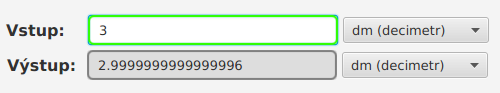
\includegraphics[width=13.5cm]{img/Chyby/Zaokrouhleni.png}
			\end{figure}
			\FloatBarrier
		
		\subsection{Převod záporné hodnoty}
		Při zadání záporné hodnoty pro převod se zobrazí chybová hláška o~záporném čísle, avšak převod se i~tak provede, viz \ref{ZapornaHodnota}.
			\begin{figure}[ht!]
				\centering
				\caption{Převod záporné hodnoty}
				\label{ZapornaHodnota}
				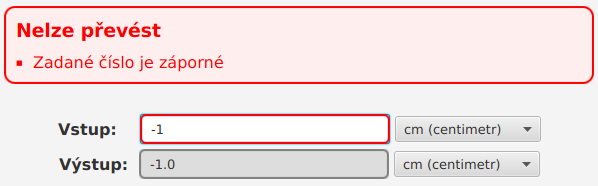
\includegraphics[width=13.5cm]{img/Chyby/ZapornaHodnota.png}
			\end{figure}
			\FloatBarrier
		
		\subsection{Tlačítko Vymaž}
		Tlačítko \emph{Vymaž} nenastaví všem komponentám výchozí hodnoty. Pouze vymaže obsah vstupního pole. Výstupní pole a~výběrové seznamy nadále obsahují hodnoty z~posledního převodu, viz \ref{Vymazani}.
			\begin{figure}[ht!]
				\centering
				\caption{Použití tlačítka Vymaž}
				\label{Vymazani}
				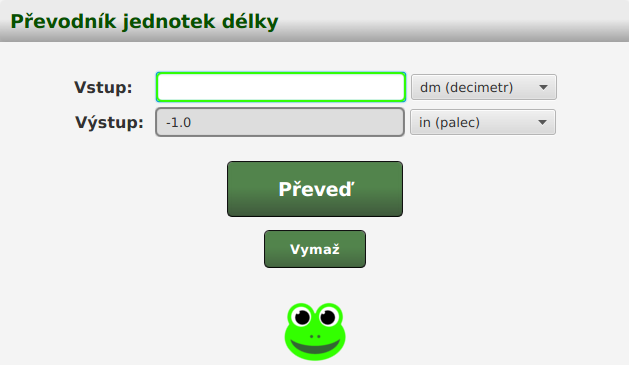
\includegraphics[width=13.5cm]{img/Chyby/Vymazani.png}
			\end{figure}